\section{Expect Outcome} \label{sec:Expect Outcome}

To evaluate our work, we design the following three scenarios and use real H.264/SVC sequences for streaming. The first two scenarios are simulated in Mininet while the third scenario use real network elements. 

\begin{figure}[tbh]
    \centering
    \begin{minipage}[t]{0.24\textwidth}
    \centering
    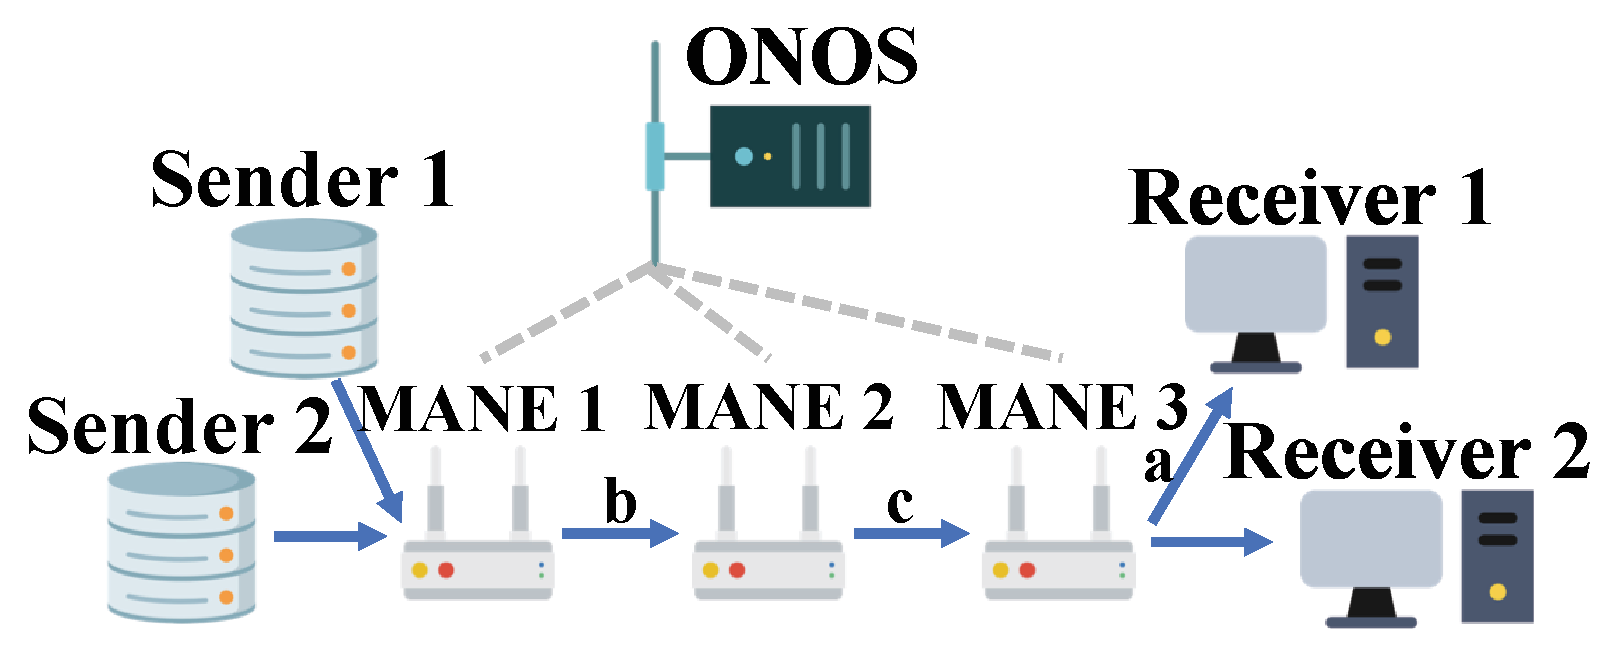
\includegraphics[width=\textwidth]{fig/scenario_2.eps}
    \caption{Mininet testbed topology (scenarios 1 and 2).}
    \label{scenario_2} 
    \end{minipage}
    \hfill\begin{minipage}[t]{0.23\textwidth}
    \centering
    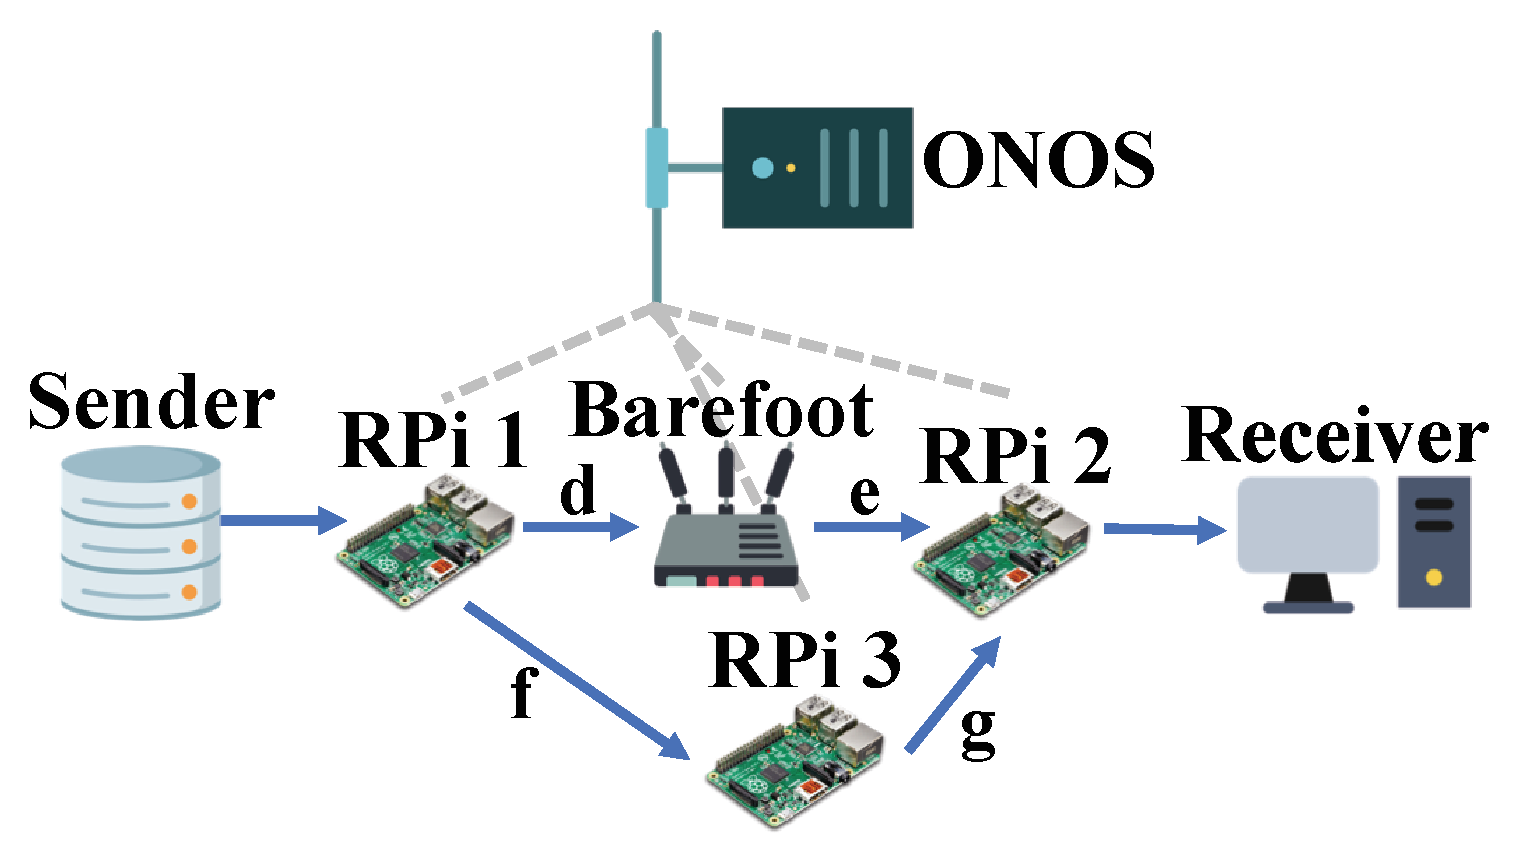
\includegraphics[width=\textwidth]{fig/scenario_3.eps}
    \caption{Real testbed topology (scenario 3).}
    \label{scenario_3} 
    \end{minipage}
\vspace{-0.1cm}
\end{figure}

\begin{itemize}
    \item{\bf Intelligent packet drops of a single video stream.}
    This is the most simple scenario with one sender, one receiver, one MANE, and one ONOS controller simulate in Mininet. We will limit the bandwidth between the nodes and make a network congestion. The MANE should detect the congestion by it's queue size. If the queue size is larger than a administrate-give number. MANE should start to drop some packets using our three logics, tail, EL, and RDO. 
    \item{\bf Optimal packet drops across multiple video streams.}
    This scenario is shown in Fig. ~\ref{scenario_2}. It is composed of multiple sender and receivers streaming multiple video sequences. This is much more difficult because we have to recognize the video sequence of the dropped packets. We evaluate the outcome among different drop logics.
    \item {\bf Error resilience with real P4 switches.}
    Fig. ~\ref{scenario_3} shows the last scenario which is composed of real network elements, some Raspberry Pi (running the reference software switch which is called $bmv2$ ~\cite{bmv2}, a software switch), a Barefoot switch, and a ONOS controller. All the links are fast Ethernet cable. Link $d$ and link $e$ are faster than link $f$ and link $g$. Therefore, the ONOS controller should add a flow through link $d$ and link $e$. Then we manually unplug link $d$ and link $e$, ONOS controller should reroute the streaming sequence through link $f$ and link $g$ so the receiver can keep receiving high-quality videos. When we plug the cable back, the ONOS controller reroutes the video stream over link $d$ and link $e$.
\end{itemize}
